\begin{frame}[t]
    \frametitle{Why MD2?}
    
    \begin{itemize}
       \item Cross-Platform approach
       \item Develop a model once, for multiple mobile platforms
       \item Decrease maintenance costs
       \item bla blub bla
    \end{itemize}
\end{frame}

\begin{frame}[t]
    \frametitle{Starting base of MD2}
    
    \begin{center}   
	    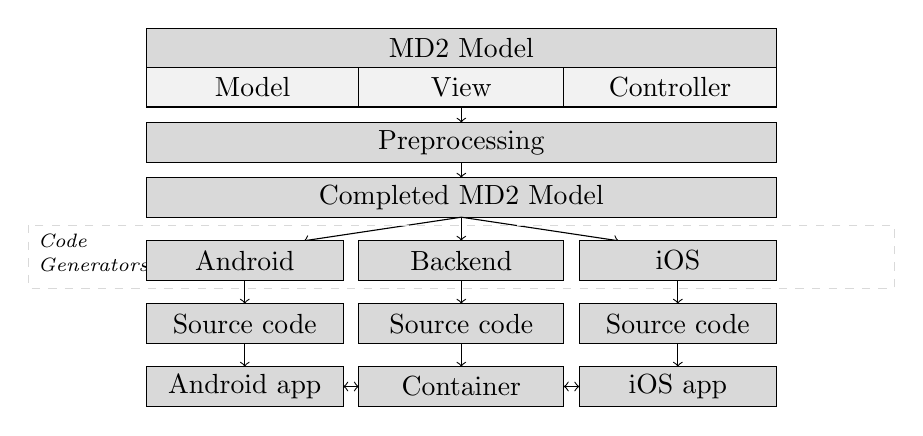
\begin{tikzpicture}
		    \draw [fill=gray!30!white] (-4,5) rectangle (4,5.5) node[pos=.5] {MD2 Model};
		    \draw [fill=gray!10!white] (-4,4.5) rectangle (-1.3,5) node[pos=.5] {Model};
		    \draw [fill=gray!10!white] (-1.3,4.5) rectangle (1.3,5) node[pos=.5] {View};
		    \draw [fill=gray!10!white] (1.3,4.5) rectangle (4,5) node[pos=.5] {Controller};
		    
		    \draw [->] (0,4.5) -- (0,4.3);
		    
		    \draw [fill=gray!30!white] (-4,3.8) rectangle (4,4.3) node[pos=.5] {Preprocessing};
		    
		    \draw [->] (0,3.8) -- (0,3.6);
		    
		    \draw [fill=gray!30!white] (-4,3.1) rectangle (4,3.6) node[pos=.5] {Completed MD2 Model};
		    
		    \draw [->] (0,3.1) -- (-2,2.8);
		    \draw [->] (0,3.1) -- (0,2.8);
		    \draw [->] (0,3.1) -- (2,2.8);
		    
		    \draw [gray!30!white, dashed] (-5.5,3) rectangle (5.5,2.2);
		    \node [right] at (-5.5,2.8) {\scriptsize{\textit{Code}}};
		    \node [right] at (-5.5,2.5) {\scriptsize{\textit{Generators}}};
		    		    
		    \draw [fill=gray!30!white] (-4,2.3) rectangle (-1.5,2.8) node[pos=.5] {Android};
		    \draw [fill=gray!30!white] (-1.3,2.3) rectangle (1.3,2.8) node[pos=.5] {Backend};
		    \draw [fill=gray!30!white] (1.5,2.3) rectangle (4,2.8) node[pos=.5] {iOS};
		    
		    \draw [->] (-2.75,2.3) -- (-2.75,2);
		    \draw [->] (0,2.3) -- (0,2);
		    \draw [->] (2.75,2.3) -- (2.75,2);
		    
		    \draw [fill=gray!30!white] (-4,1.5) rectangle (-1.5,2) node[pos=.5] {Source code};
		    \draw [fill=gray!30!white] (-1.3,1.5) rectangle (1.3,2) node[pos=.5] {Source code};
		    \draw [fill=gray!30!white] (1.5,1.5) rectangle (4,2) node[pos=.5] {Source code};
		    
		    \draw [->] (-2.75,1.5) -- (-2.75,1.2);
		    \draw [->] (0,1.5) -- (0,1.2);
		    \draw [->] (2.75,1.5) -- (2.75,1.2);
		    
		    \draw [fill=gray!30!white] (-4,0.7) rectangle (-1.5,1.2) node[pos=.5] {Android app};
		    \draw [fill=gray!30!white] (-1.3,0.7) rectangle (1.3,1.2) node[pos=.5] {Container};
		    \draw [fill=gray!30!white] (1.5,0.7) rectangle (4,1.2) node[pos=.5] {iOS app};	
		    
		    \draw [<->] (-1.5,0.95) -- (-1.3,0.95); 
		    \draw [<->] (1.5,0.95) -- (1.3,0.95);    
		    
	    \end{tikzpicture}
    \end{center}
    
{\color{gray}{\tiny{Source: MD2 Project Seminar Presentation}}}

\end{frame}



\begin{frame}[t]
    \frametitle{Project Goals}
    
    \begin{itemize}
       \item Implement and extend generator for map.apps platform
       \item bla blub bla
    \end{itemize}
\end{frame}


